\section{Sequenzdiagramme}

\subsection{Hinzufügen eines Knotens}
\begin{figure}[h!]
\begin{center}
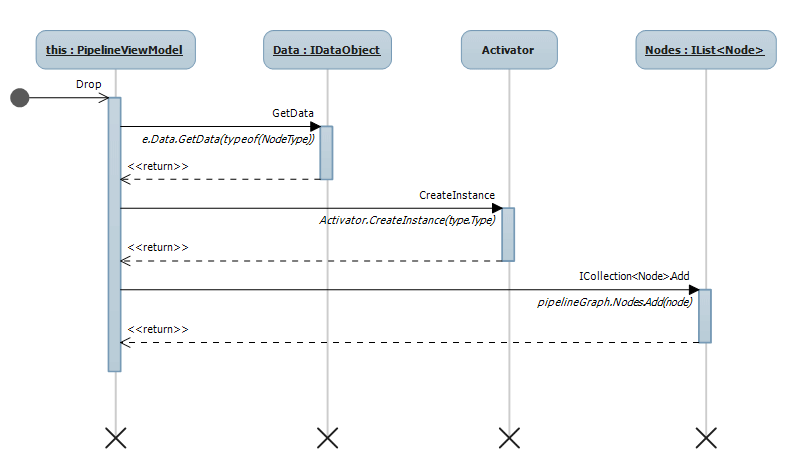
\includegraphics[width=0.8\textheight,angle=90]{Diagrams/drop.png}
\end{center}
\end{figure}
\newpage

\begin{description}
	\item[Vorraussetzung] Das Programm ist gestartet.
	\item[äußerer Ablauf] Der Benutzer erzeugt einen beliebigen Knoten, indem er ihn per ``Drag-and-Drop'' aus einer am unteren Bildschirmrand angebrachten Leiste zieht.
	\item[innerer Ablauf] Durch das Platzieren des Knotens im Pipeline Graph wird ein Drop-Ereignis erzeugt. Dieses wird vom PipelineViewModel verarbeitet, indem zunächst die Art des platzierten Knotens erfasst und danach eine neue Instanz dieses Knotentyps erzeugt wird. Anschließend wird der neue Knoten zu der vom Pipeline Graph gehaltenen Liste der momentan vorhandenen Knoten hinzugefügt.
\end{description}
\newpage
\subsection{Hinzufügen eines Ausgabefensters}
\begin{figure}[h!]
\begin{center}
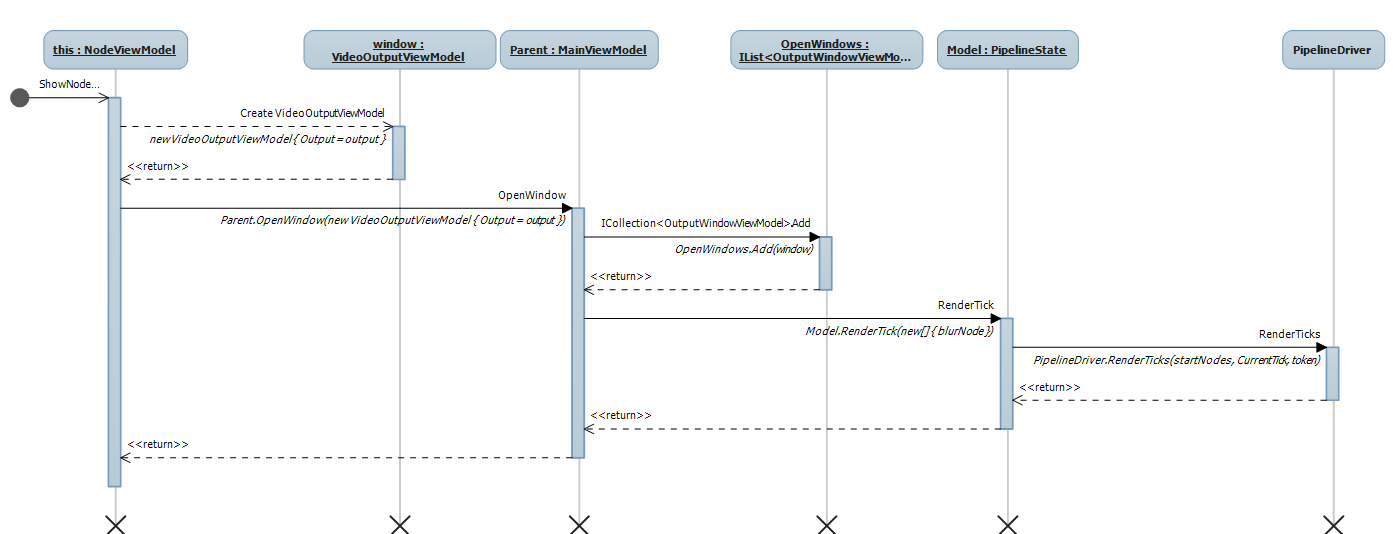
\includegraphics[width=0.9\textheight,angle=90]{Diagrams/shownodeoutput.png}
\end{center}
\end{figure}
\newpage

\begin{figure}[h!]
\begin{center}
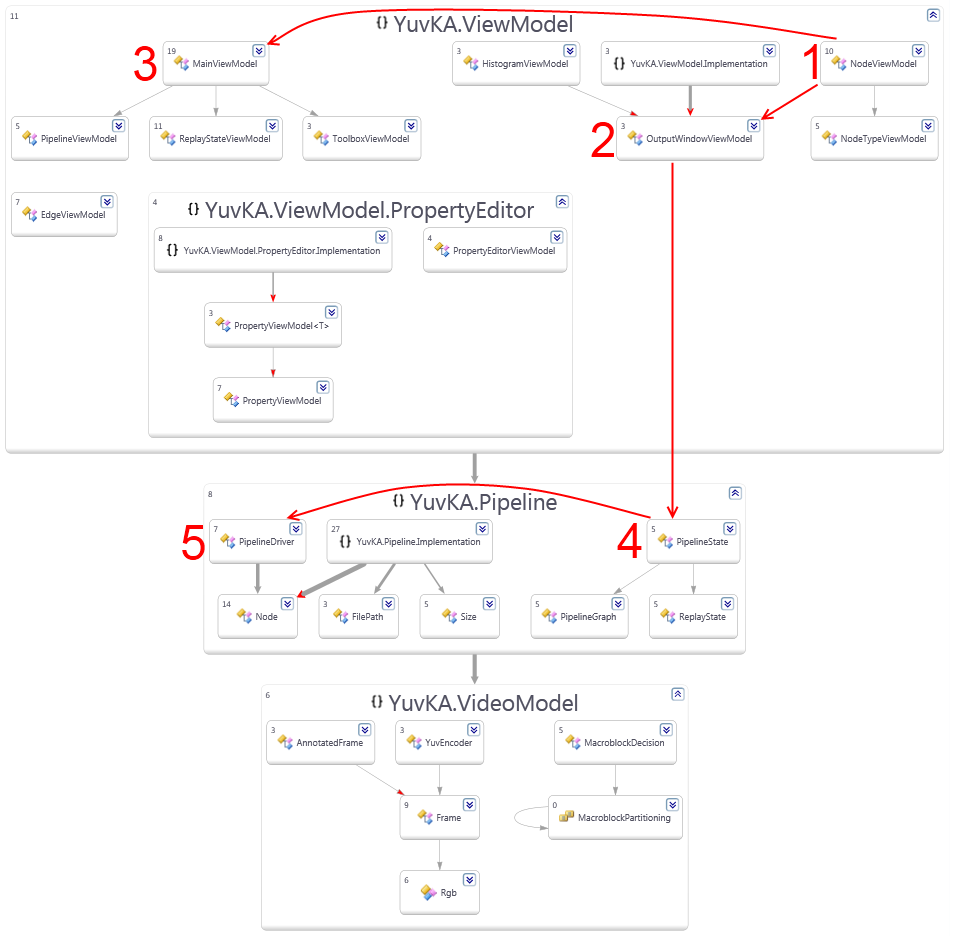
\includegraphics[width=0.9\textwidth]{Diagrams/visualization_TC2.png}
\end{center}
\caption{Veranschaulichung des Ablaufs anhand des Klassendiagramms}
\end{figure}
\begin{description}
	\item[Vorraussetzung] Der Benutzer hat eine Pipeline gebaut, die einen Weichzeichnungsknoten enthält.
	\item[äußerer Ablauf] Der Benutzer ruft das Kontextmenü des Weichzeichnungsknotens auf und wählt die Option ``Video anzeigen".
	\item[innerer Ablauf] Der Aufruf der Option wird vom NodeViewModel (1) verarbeitet. Dieses erstellt ein neues VideoOutput Fenster, verwaltet vom VideoOutputViewModel (2). Dieses Fenster wird vom MainViewModel (3) in dessen Liste aller geöffneten Fenster aufgenommen. Zum Abspielen ruft das MainViewModel die Klasse ReplayState (4) auf. Diese wiederum benutzt den PipelineDriver (5, siehe auch nächstes Diagramm) zum Verarbeiten des Videos.
\end{description}
\newpage
\subsection{Abspielen der Pipeline}
\begin{figure}[h!]
\begin{center}
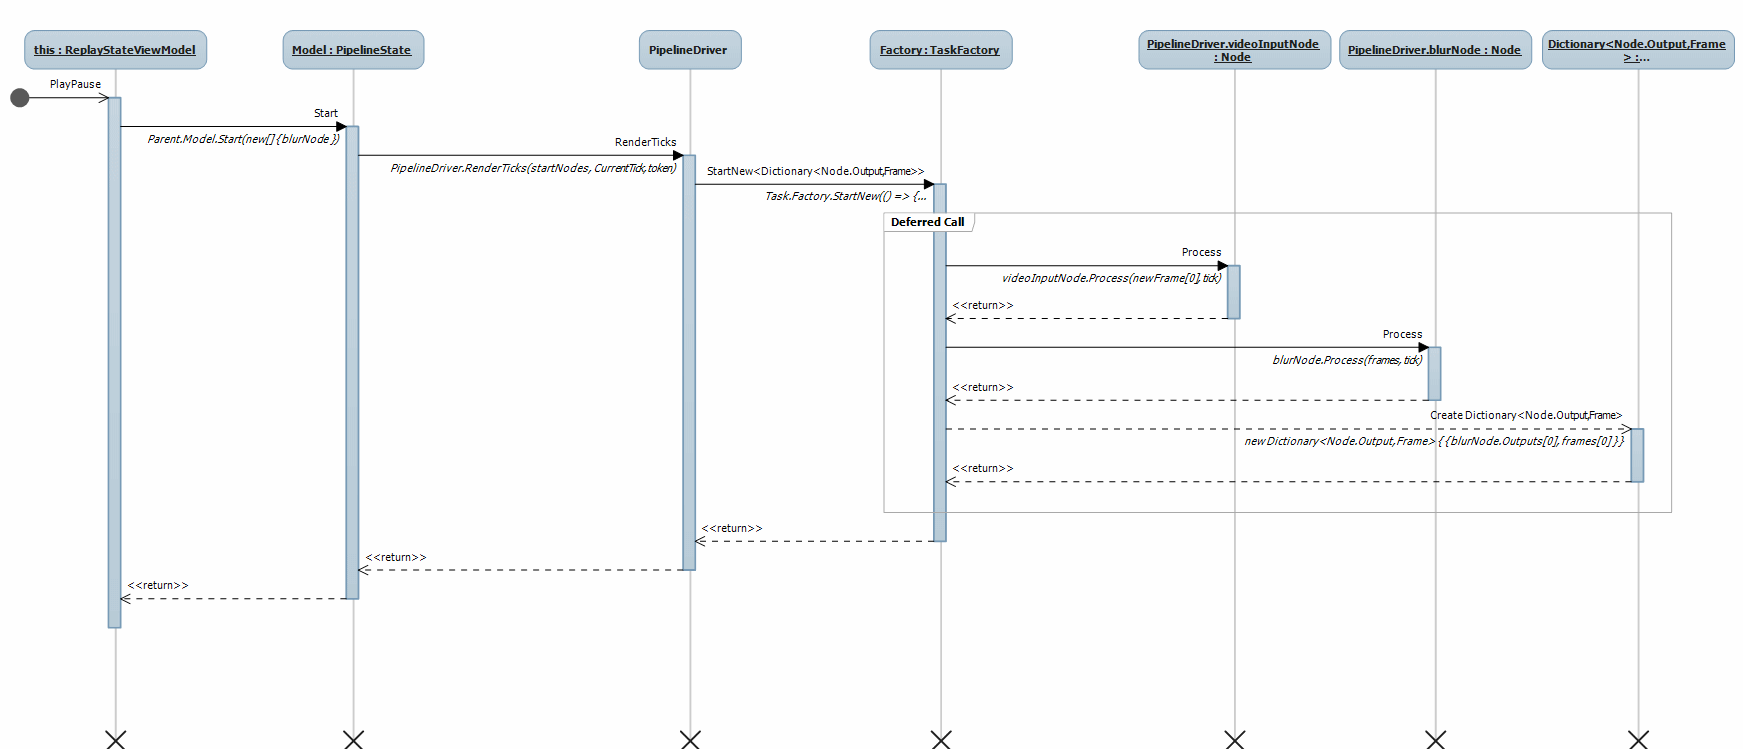
\includegraphics[width=0.9\textheight,angle=90]{Diagrams/play.png}
\end{center}
\end{figure}
\newpage

\begin{figure}[h!]
\begin{center}
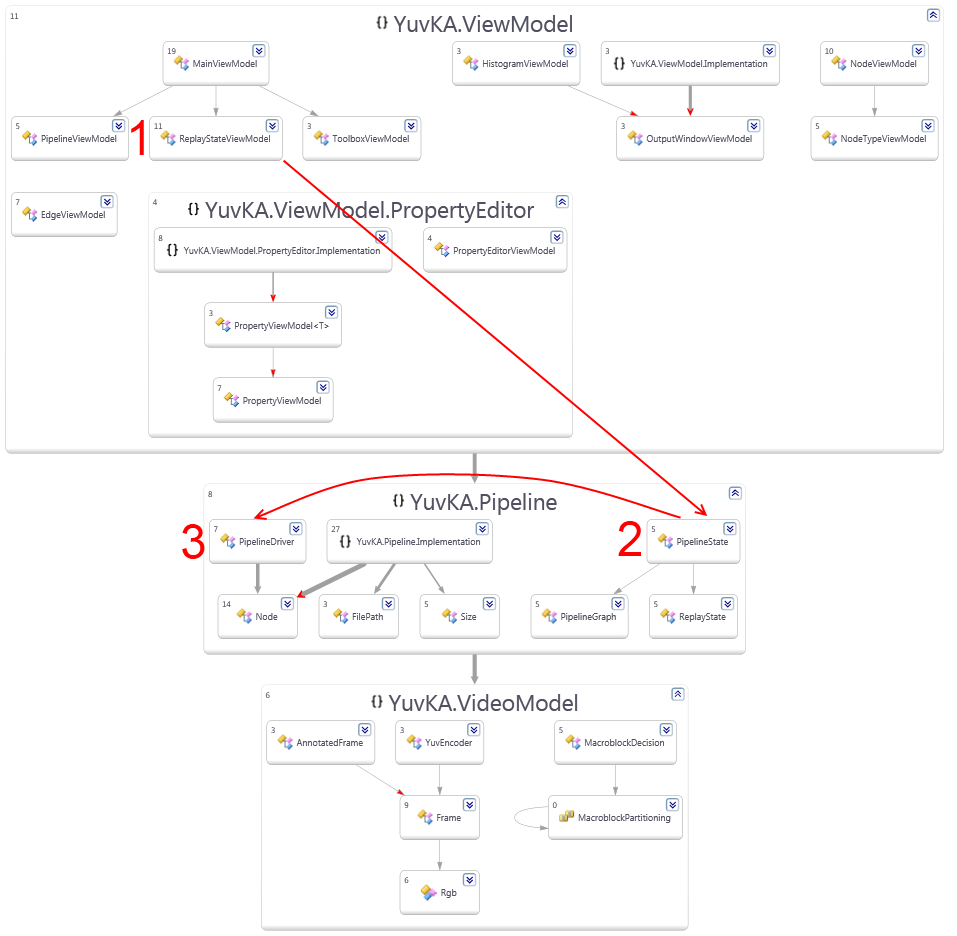
\includegraphics[width=0.9\textwidth]{Diagrams/visualization_TC3.png}
\end{center}
\caption{Veranschaulichung des Ablaufs anhand des Klassendiagramms}
\end{figure}
\begin{description}
	\item[Vorraussetzung] Der Benutzer hat eine Pipeline gebaut, die einen Weichzeichnungsknoten enthält und dessen Ausgabefenster geöffnet.
	\item[äußerer Ablauf] Der Benutzer drückt auf den Play-Knopf, um die Pipeline abzuspielen.
	\item[innerer Ablauf] Der Aufruf der Option wird vom ReplayStateViewModel (1) verarbeitet. Zum Abspielen ruft es  über das MainViewModel die Klasse ReplayState (2) auf. Diese wiederum benutzt den PipelineDriver (3) zum Verarbeiten des Videos. Der PipelineDriver verarbeitet die Frames, indem er für jeden Knoten einen Thread erstellt und diese nacheinander das Video abarbeiten lässt.
\end{description}
